\chapter{Methodology/Design/Implementation}
\label{chapter:method}
\section{Phase Locked Loop System Overview}
\label{sec:pll_overview}
A Phase-Locked Loop (PLL) is a negative feedback control system circuit. As the name implies, the purpose of a PLL is to generate a signal whose phase matches that of a reference signal. This is achieved through multiple iterations of comparing the reference and feedback signals (ref fig:\ref{fig:pll_1}). The overall goal of the PLL is to align the phases of the reference and feedback signals—this is referred to as the lock mode. Once locked, the PLL continues to compare the two signals, but since they are in lock mode, the PLL output remains constant. \\
\textbf{A basic PLL consists of four main components:}
\begin{enumerate}
	\item Phase Detector or Phase Frequency Detector (PD or PFD)
	\item Charge Pump (CP)
	\item Low Pass Filter (LPF)
	\item Voltage-Controlled Oscillator (VCO)
\end{enumerate}
The Phase Frequency Detector (PFD) measures the phase difference between the reference and feedback signals. If a phase difference exists, it generates synchronized “up” or “down” signals to the charge pump and low pass filter. If the error signal from the PFD is an “up” signal, the charge pump adds charge to the LPF capacitor, increasing the control voltage, \( V_{\text{cntrl}} \). Conversely, if the error signal is a “down” signal, the charge pump removes charge from the LPF capacitor, decreasing \( V_{\text{cntrl}} \).\tikzstyle{block} = [draw, rectangle]
\tikzstyle{input} = [coordinate]
\tikzstyle{output} = [coordinate]
\tikzstyle{pinstyle} = [pin edge={to-,thin,black}]
\begin{figure}[h]
    \centering
    \begin{tikzpicture}[
      block/.style={draw, thick, minimum width=3cm, minimum height=2.5cm, align=center},
      line/.style={-Stealth, thick},
      node distance=1.5cm and 1.5cm
    ]
    
    % Blocks
    \node[input,name=inputref] (input) {fref};
    \node[block, right=2cm of input] (pd) {PD};
    \node[block, right of=pd] (cp) {CP};
    \node[block, right of=cp] (vco) {VCO};
    \node[block, below of=cp , node distance=1cm] (lpf) {LPF};
    
% Signals
\coordinate[left=1.5cm of pd] (inputref);
\coordinate[below=0cm of inputref] (inputfb);
\coordinate[right=1.5cm of vco] (output);
    
    % Connections
    % \draw [->] (inputref) -- node {$fref$} (pd);
    % \draw[--] (inputref) node[left] {$f_{ref}$} -- (pd);
    % \draw[--] (inputfb) node[left] {$f_{fb}$} -- (pd);
    \draw[line] ( inputref) -- node[above] {$f\_ref$} (pd);
    \draw[line] (inputfb) -- node[above] {$f\_fb$} ([yshift=2cm]pd);
    % \draw[--] (pd) -- (cp);
    % \draw[line] (cp) -- node[above] {$V_{cntrl}$} (vco);
    % \draw[line] (cp) |- (lpf);
    % \draw[line] (lpf) -| (vco);
    
    % \draw[line] (vco) -- node[above] {$f_{out}$} (output);
    % \draw[line] (output) |- ++(0,-2) -| (inputfb);
    
    \end{tikzpicture}
    \caption{PLL Block Diagram}
\end{figure}\\
The control voltage \( V_{\text{cntrl}} \) serves as the input to the VCO. The LPF is essential for allowing only DC signals into the VCO and for storing the charge from the CP. The VCO adjusts the feedback signal's frequency based on the error generated by the PFD. If the PFD generates an “up” signal, the VCO speeds up the feedback signal. Conversely, if a “down” signal is generated, the VCO slows it down. The output of the VCO is then fed back to the PFD to recalculate the phase difference, thereby creating a closed-loop frequency control system.

\subsection{Phase Detector}
A phase detector is a circuit that detects the difference in phase between its two input
signals. An example of a basic phase detector is the XOR gate. It produces error pulses on both
falling and rising edges.

\begin{figure}[!h]
\centering
\resizebox{0.3\textwidth}{!}{%
\begin{circuitikz}
\tikzstyle{every node}=[font=\huge]
% \draw (11.75,11.25) to[short] (12.25,11.25);
% \draw (11.75,10.75) to[short] (12.25,10.75);
\draw (12.25,11.25) node[ieeestd xor port, anchor=in 1, scale=1](port){} (port.out) to[short] (14.25,11);
\node [font=\LARGE] at (11.25,11.5) {$\phi_{\text{ref}}$};
\node [font=\LARGE] at (11.25,10.75) {$\phi_{\text{vco}}$};
\end{circuitikz}
}%
\label{fig:xor_gate}
\caption{}
\end{figure}
\subsubsection{Phase Frequency Detector}
A phase frequency detector (PFD) is a circuit that detects the difference in phase and frequency between its two input signals. PFD is a more advanced version of the basic phase detector. It can detect both phase and frequency differences, making it more suitable for applications where the input signals may have different frequencies. The PFD generates an error signal that is proportional to the phase and frequency difference between the two input signals. This error signal is then used to control the charge pump and low pass filter in the PLL.
\begin{figure}[h]
    \centering
    \resizebox{0.8\textwidth}{!}{%
    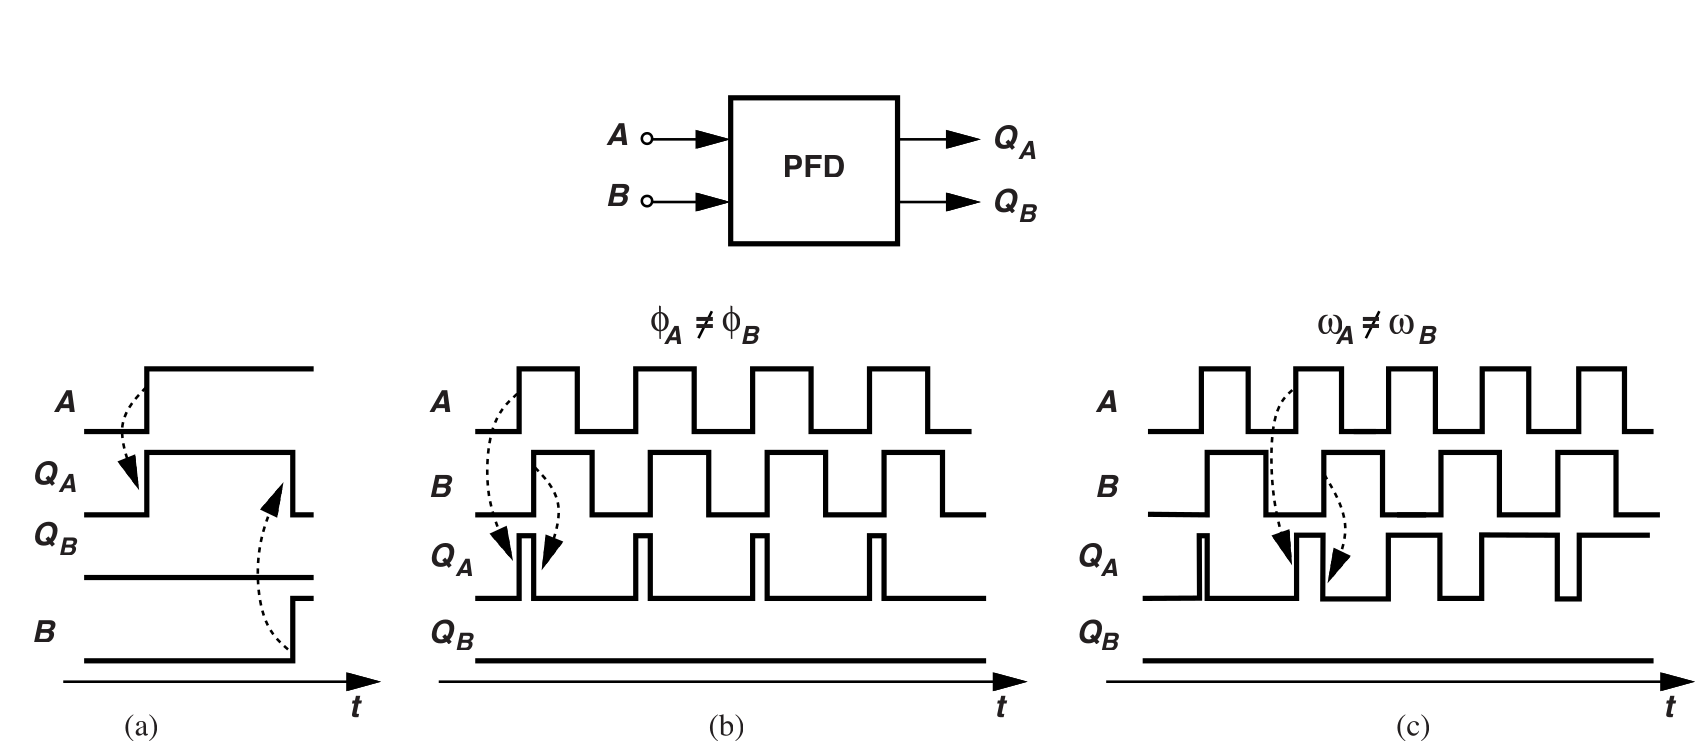
\includegraphics{figs/pfd_block.png}
    }%
    \caption{(a) Conceptual PFD operation, (b) case of input phase difference, and (c) case of input frequency difference}
    \label{fig:pfd_block}
\end{figure}

PFD state diagram is shown in Figure \ref{fig:pfd_state_diagram}. 
The PFD circuit is a sequential circuit which produces UP and DOWN outputs which inform the CP to charge or discharge the loop
filter depending on the phase difference between the two input signals of PFD. Depending on which signal becomes high first, the REF signal or the FB signal in Figure \ref{fig:pfd_state_diagram}, the circuit goes either to state 1 or to state 2. Supposing the circuit goes to state 1, if the FB signal becomes high, the circuit goes back to state 0. The longer it takes the FB to transit to 1, the longer will UP high signal remain high. This wider pulse on the other hand serves as a control voltage for the CP. The bigger the width of the UP signal, the greater the input voltage to the VCO will be, increasing the frequency of the output signal. Basically, the circuits let the CP know if the phase of the Frequency Divider (FD) circuit is higher or lower than some reference signal and helps to discharge or charge the node right after the CP circuit. If the frequency of the input signal is higher than the frequency of the output signal, the circuit will only go from state 0 to state 1 and will keep charging up the LF. On the other scenario, if the input frequency is lower than the output frequency, the output of the CP will be discharged leading to reduced frequencies on the VCO circuit.

\begin{figure} [!h]
    \centering
    \resizebox{0.8\textwidth}{!}{%
    

% \begin{tikzpicture}[->, >=stealth', auto, node distance=3.5cm, semithick]
% \tikzstyle{every state}=[draw=black, thick, fill=gray!10, minimum size=1.2cm]

% % Nodes
% \node[state] (S1) {UP=0\\DN=1};
% \node[state, right of=S1] (S2) {UP=0\\DN=0};
% \node[state, right of=S2] (S3) {UP=1\\DN=0};

% % Transitions
% \path 
% (S1) edge[loop left] node[align=center]{FB ↑} (S1)
% (S1) edge[bend left] node{REF ↑} (S2)
% (S2) edge[bend left] node{FB ↑} (S1)
% (S2) edge[bend left] node{REF ↑} (S3)
% (S3) edge[bend left] node{FB ↑} (S2)
% (S3) edge[loop right] node[align=center]{REF ↑} (S3);

% \end{tikzpicture}
\begin{tikzpicture}[node distance=3cm]
    \node[state] (q1) {a};
    \node[state, right of =q1] (q2) {b};
    \node[state, right of = q2] (q3) {c};
    % \node[state] (q2) [side of= q1] {locked};
\end{tikzpicture}
    
    }%
    \caption{PFD state diagram}
    \label{fig:pfd_state_diagram}
    % \vspace{-0.5cm}
\end{figure}

This PFD circuit senses the 0 to 1 transitions of VREF and VFB and produces UP and DOWN signals depending on which of the input signal rises quicker. Theoretically, this is a very easy circuit to be build and it should work very close to the ideal circuit.
One of the problems that is faced in real PFD blocks is the dead-zone of the PFD which happens for very small phase differences. The block diagram of PFD is shown in \ref{fig:pfd_dff_blk}
\begin{figure}[h]
	\centering
	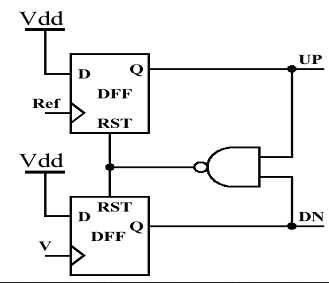
\includegraphics[width=0.5\textwidth]{figs/pfd_dff_blk.png}
	% \vspace{-0.3cm}
	\caption{PFD circuit using D flip-flops}
	\label{fig:pfd_dff_blk}
	\vspace{0.5cm}
\end{figure}
\subsection{Nanda biceps Pump}
The charge pump is a circuit that converts the error signal from the phase detector into a control voltage for the VCO. The charge pump consists of two switches and a capacitor. The switches are controlled by the error signal from the phase detector. When the error signal is high, the switch connects the capacitor to the power supply, charging it. When the error signal is low, the switch connects the capacitor to ground, discharging it. The control voltage for the VCO is taken from the capacitor.
\begin{figure}[!ht]
    \centering
    \resizebox{0.2\textwidth}{!}{%
    \begin{circuitikz}
    \tikzstyle{every node}=[font=\large]
    
    
    \draw [ line width=0.6pt](10.75,16) to[american current source,l={ \large Icp}] (10.75,14);
    \draw [ line width=0.6pt](10.75,11.75) to[american current source,l={ \large Icp}] (10.75,9.5);
    \draw [line width=0.6pt](10.75,11.75) to[normal open switch] (10.75,12.5);
    \draw [line width=0.6pt](10.75,12.5) to[normal open switch] (10.75,14);
    \draw [line width=0.6pt](10.75,9.75) to (10.75,9.5) node[ground]{};
    \draw [ line width=0.6pt](10.25,16) to[short] (11.25,16);
    \draw [ line width=0.6pt](10.75,12.75) to[short, -o] (12,12.75) ;
    \draw [ line width=0.6pt](10.75,12) to[short, -o] (9.25,12) ;
    \draw [ line width=0.6pt](10.75,13.25) to[short, -o] (9.25,13.25) ;
    \node [font=\large] at (12.5,13) {Iout};
    \node [font=\large] at (8.25,13.25) {Up};
    \node [font=\large] at (8.5,12) {Down};
    \end{circuitikz}
    }%
    
    \label{fig:my_label}
\end{figure}

The CP circuit should ideally behave as in Table~
\ref{tab:cp_function}.

\begin{table}[h!]
\centering
\begin{tabular}{|c|c|c|}
\hline
\textbf{UP} & \textbf{DOWN} & \textbf{IOUT} \\
\hline
0 & 0 & 0 \\
0 & 1 & $-\text{I}_{\text{CP}}$ \\
1 & 0 & $+\text{I}_{\text{CP}}$ \\
1 & 1 & 0 \\
\hline
\end{tabular}
\caption{Charge Pump Functionality.}
\label{tab:cp_function}
\end{table}

\subsection{Low Pass Filter}
The low pass filter is a circuit that removes high frequency noise from the control voltage generated by the charge pump. The low pass filter consists of a resistor and a capacitor. The resistor limits the current flowing into the capacitor, while the capacitor stores the charge. The output of the low pass filter is a smooth control voltage that is fed to the VCO.
% \input{figs/lpf.tex}


\subsection{Voltage Controlled Oscillator}
The voltage controlled oscillator (VCO) is a circuit that generates an output signal whose frequency is proportional to the control voltage. The VCO consists of a transistor and a capacitor. The transistor is biased by the control voltage, which determines its operating frequency. The output of the VCO is fed back to the phase detector to complete the PLL loop.
\begin{equation}
	\label{eq:vco_char}
	f_{out} = K_{vco} * V_{in} + f_{min}
\end{equation}
\begin{figure}[h]
    \begin{subfigure}[][][1]{0.5\textwidth}
        \centering
    \resizebox{1\textwidth}{!}{%
    \begin{circuitikz}
    \tikzstyle{every node}=[font=\Large]
    
    
    \draw [ line width=0.6pt ] (8,16.5) rectangle  node {\Large VCO} (13.25,13.25);
    \draw [->, >=Stealth] (6.75,15) -- (8,15);
    \draw [->, >=Stealth] (13.25,15) -- (14.75,15);
    \node [font=\Large] at (5.5,15) {$V_{Cntrl}(V_{C})$};
    \node [font=\Large] at (15.3,15) {$f_{out}$};
    \end{circuitikz}
    }%
    \end{subfigure}
    \begin{subfigure}[][][1]{0.5\textwidth}
        \centering
            \centering
            \begin{tikzpicture}[
                axis/.style={->, thick},
                dashedline/.style={dashed, thick},
                solidline/.style={thick},
                font=\small,
                scale=1.2
            ]
            
            % Axes
            \draw[axis] (0,0) -- (6,0) node[right] {$V_C$};
            \draw[axis] (0,0) -- (0,5) node[above] {$f$};
            
            % Coordinates
            \coordinate (Vcmin) at (1,0);
            \coordinate (Vcnom) at (3,0);
            \coordinate (Vcmax) at (5,0);
            
            \coordinate (fcmin) at (0,1);
            \coordinate (fcnom) at (0,3);
            \coordinate (fcmax) at (0,4.5);
            
            \coordinate (p1) at (1,1);
            \coordinate (p2) at (3,3);
            \coordinate (p3) at (5,4.5);
            
            % Vertical dashed lines
            \draw[dashedline] (Vcmin) -- (p1);
            \draw[dashedline] (Vcnom) -- (p2);
            \draw[dashedline] (Vcmax) -- (p3);
            
            % Horizontal dashed lines
            \draw[dashedline] (fcmin) -- (p1);
            \draw[dashedline] (fcnom) -- (p2);
            \draw[dashedline] (fcmax) -- (p3);
            
            % VCO Line
            \draw[solidline] (p1) -- (p3);
            
            % Labels
            \node[below] at (Vcmin) {$V_{C(\min)}$};
            \node[below] at (Vcnom) {$V_{C(\text{nom})}$};
            \node[below] at (Vcmax) {$V_{C(\max)}$};
            
            \node[left] at (fcmin) {$f_{o(\min)}$};
            \node[left] at (fcnom) {$f_{o(\text{nom})}$};
            \node[left] at (fcmax) {$f_{o(\max)}$};
            
            \end{tikzpicture}
    \end{subfigure}            
    \caption{VCO Block Diagram and Characteristics}
    \label{fig:vco_block}
    % \vspace{-0.5cm}
\end{figure}
The VCO transfer function can be given as
\begin{equation}
	\label{eq:vco_tf}
	H_{vco}(s) = \frac{\phi_{o}(s)}{v_{o}(s)} = \frac{K_{vco}}{S}
\end{equation}
The gain of the voltage-controlled oscillator is simply the slope of the curves given in Fig.\ref{fig:vco_block}. This gain can be written as
\begin{equation}
	\label{eq:vco_gain}
	K_{vco} = 2\pi  * \frac{f_{max} - f_{min}}{V_{max} - V_{min}}(radians/s * V)
\end{equation}
Kvco is an important factor it Determines the PLL settling time.
There are different types of VCO like : Cross Coupled LC VCO, Current Starved VCO, Colpitts Oscillator. For this project, Current Starved VCO is used.
\subsection{Frequency Divider}
The frequency divider is a circuit that divides the frequency of the output signal from the VCO by a fixed integer value. The frequency divider is used to reduce the frequency of the output signal to match the frequency of the reference signal. The frequency divider can be implemented using a flip-flop or a counter. The output of the frequency divider is fed back to the phase detector to complete the PLL loop.
\subsubsection*{Frequency Divider Principle}
A frequency divider works by toggling the output state of a flip-flop at each rising (positive) edge of the input clock signal. A single flip-flop divides the frequency of the input clock by a factor of 2. Cascading multiple flip-flops results in further division:
\begin{equation}
	\label{eq:freq_div}
	f_{\text{out}} = \frac{f_{\text{in}}}{2^n}
\end{equation}
Where:
\begin{itemize}
    \item $f_{\text{in}}$ is the input clock frequency,
    \item $f_{\text{out}}$ is the output frequency after division,
    \item $n$ is the number of flip-flops connected in series.
\end{itemize}
\subsubsection*{Positive Edge-Triggered Flip-Flop}
A positive edge-triggered flip-flop changes its output state only at the rising edge of the clock signal. A T (toggle) flip-flop toggles its output on each clock edge. However, a D flip-flop can be configured to behave as a T flip-flop by connecting the inverted output back to the input:
\[
D = \sim Q
\]
This ensures the flip-flop toggles its output on each positive clock edge.
\subsubsection*{Implementation Using Pass Gates and Inverters}
A D flip-flop can be constructed using two D latches in a master-slave configuration, controlled by a clock and its complement. Each latch consists of pass gates and inverters.
\begin{itemize}
    \item Pass gates (transmission gates) are used to control the flow of data based on the clock signal. They are bidirectional switches typically made using a combination of NMOS and PMOS transistors.
    \item Inverters act as buffers and memory elements to store and propagate the logic state.
\end{itemize}
\subsubsection*{Frequency Division Design Circuit Using LT Spice}

\subsubsection*{Positive Edge-Triggered Flip-Flop}
A positive edge-triggered flip-flop changes its output state only at the rising edge of the clock signal. A T (toggle) flip-flop toggles its output on each clock edge. However, a D flip-flop can be configured to behave as a T flip-flop by connecting the inverted output back to the input:
\[
D = \sim Q
\]
This ensures the flip-flop toggles its output on each positive clock edge.
\subsubsection*{Implementation Using Pass Gates and Inverters}
A D flip-flop can be constructed using two D latches in a master-slave configuration, controlled by a clock and its complement. Each latch consists of pass gates and inverters.
\begin{itemize}
    \item Pass gates (transmission gates) are used to control the flow of data based on the clock signal. They are bidirectional switches typically made using a combination of NMOS and PMOS transistors.
    \item Inverters act as buffers and memory elements to store and propagate the logic state.
\end{itemize}
\subsubsection*{Frequency Division Design Circuit Using LT Spice}
To design a frequency divider circuit in LT Spice, follow these steps:
\begin{itemize}
    \item Create a schematic with a clock source and a D flip-flop.
    \item Configure the D flip-flop to toggle on each clock edge by connecting its inverted output back to the input.
    \item Simulate the circuit to observe the frequency division at the output.
    \item For cascading, connect the output of one flip-flop to the clock input of the next stage.
\end{itemize}
\subsubsection*{Working Principle}
\begin{itemize}
    \item When CLK = 1, the master latch is transparent and allows input data to propagate, while the slave latch holds its state.
    \item When CLK = 0, the master latch latches the input data, and the slave latch becomes transparent to pass the stored value to the output.
    \item This configuration ensures that data is transferred to the output only on the rising edge of the clock, making it a positive edge-triggered flip-flop.
\end{itemize}
\subsubsection*{Frequency Division Operation}
By cascading multiple such flip-flops, a frequency divider circuit is realized. The output of each flip-flop acts as the clock for the next stage. Since each stage toggles at half the frequency of the previous one, the overall division factor is \(2^n\).

For example:
\begin{itemize}
    \item 1 Flip-Flop → Divide by 2
    \item 2 Flip-Flops → Divide by 4
    \item 3 Flip-Flops → Divide by 8
\end{itemize}
\begin{figure}[H] % Use 'H' specifier for strict placement
    \centering
    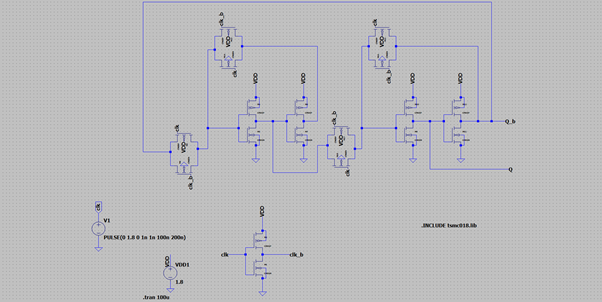
\includegraphics[width=0.8\textwidth]{figs/circuit.png}
    \caption{Frequency Divider Circuit}
    \label{fig:LT Spice Circuit}
\end{figure}
The schematic shown in the figure represents a frequency divider circuit designed using positive edge-triggered D flip-flops. The circuit is implemented at the transistor level using pass gates (transmission gates) and inverters, which are fundamental components in CMOS logic design. This implementation provides a realistic view of how sequential circuits function at a lower abstraction level, offering better understanding of timing, logic flow, and hardware behavior.
The design uses a PULSE voltage source to generate the clock signal. This source is defined to oscillate between 0V and 1.8V with 1 ns rise and fall times, a pulse width of 100 ns, and a time period of 300 ns. The generated clock signal (clk) is used to drive the flip-flops in the circuit. An inverter is used to create the complementary clock signal (clk\_b), which is necessary to properly control the pass gates in the master-slave latch configuration of each D flip-flop.

Each flip-flop is constructed using two D latches connected in a master-slave configuration. Each latch consists of a pair of transmission gates, controlled by the clock and its complement, and inverters, which serve to store and propagate the logic state. This structure ensures that the flip-flop captures input data only on the rising edge of the clock signal, making it a positive edge-triggered flip-flop. To make the flip-flops function as T (toggle) flip-flops, the inverted output (\(Q_b\)) is fed back to the D input of each flip-flop. This feedback ensures that the flip-flop toggles its output on every rising edge of the clock.

In this circuit, two flip-flops are cascaded to form a 2-stage frequency divider. The first flip-flop toggles its output on every clock cycle, effectively dividing the input frequency by 2. The second flip-flop receives the output of the first as its clock input and toggles on every rising edge of that signal, thereby dividing the frequency by another factor of 2. As a result, the final output signal has a frequency equal to one-fourth of the original input clock. This cascading approach can be extended to more stages for greater frequency division.

The simulation is performed using SPICE, with the \texttt{.tran 100u} command specifying a transient analysis over a period of 100 microseconds to observe the dynamic behavior of the circuit. The schematic also includes a reference to a process design kit (\texttt{.INCLUDE tsmc018.lib}), which models the behavior of transistors based on the TSMC 180nm CMOS technology. This provides accurate transistor-level simulation results, allowing verification of correct operation and timing characteristics.

In conclusion, the schematic demonstrates the design and working of a CMOS-based frequency divider using positive edge-triggered D flip-flops implemented with pass gates and inverters. It effectively divides the clock frequency by powers of two and can be used in a variety of digital systems requiring timing control, clock scaling, or counter functionality.

\begin{figure}[H] % Use 'H' specifier for strict placement
    \centering
    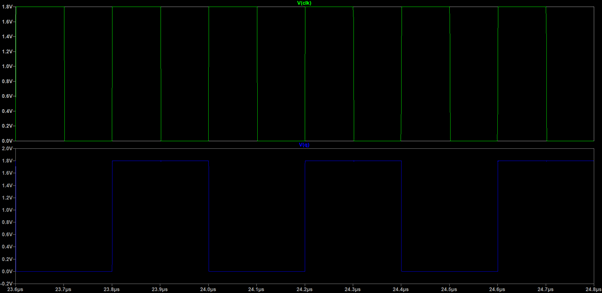
\includegraphics[width=0.8\textwidth]{figs/waveform.png}
    \caption{Frequency Divider Output Waveform}
    \label{fig:Output Waveform}
\end{figure}
\subsubsection*{Conclusion}
In this project, a frequency divider circuit was successfully designed and implemented using positive edge-triggered D flip-flops constructed with pass gates and inverters. The use of transistor-level design under TSMC 180nm CMOS technology provided a deeper understanding of the internal working of sequential circuits. Simulation results verified that each flip-flop stage effectively divides the input clock frequency by a factor of two. This design is efficient for low-power, high-speed digital systems and demonstrates the practical use of basic building blocks in creating complex timing circuits.

\subsubsection*{Applications}
\begin{itemize}
    \item \textbf{Clock Division in Microprocessors:} Used to generate lower frequency clocks from a high-speed master clock.
    \item \textbf{Digital Watches and Timers:} Essential for time base generation.
    \item \textbf{Pulse Generation Circuits:} Helps in creating precise timing pulses for control systems.
    \item \textbf{Frequency Synthesizers:} Used in communication systems to derive required frequencies.
\end{itemize}
\section{Design of PLL blocks}
The numberous block have been designed for the PLL taking in consideration of the practical aspects.
\subsection{PFD Design}
As shown in figure \ref{fig:pfd_dff_blk}, PFD circuit requires two D flip-flops, and one AND gate. A very fast RESET is required in order to reduce the PFD dead-zone.Hence it limits the reference frequency at which the pll can be clocked at.Here to overcome the dead zone issue we have implemented a nand based pfd.
% \begin{figure}
% 	\centering
% 	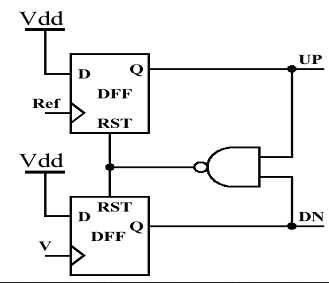
\includegraphics[width=0.5\textwidth]{figs/pfd_dff_blk.png}
% 	% \vspace{-0.3cm}
% 	\caption{PFD circuit using D flip-flops}
% 	\label{fig:pfd_dff_blk}
% 	\vspace{0.5cm}
% \end{figure}
\subsubsection{2 intput NAND gate}
The 2 input NAND gate is implement in static CMOS logic. The circuit is made using 4 transistors, 2 PMOS and 2 NMOS. The PMOS transistors are connected in parallel and the NMOS transistors are connected in series. The output of the NAND gate is taken from the drain of the NMOS transistors.
\subsubsection{3 input NAND gate}
\subsubsection{4 input NAND gate}
\subsubsection{inverter}
\subsubsection{NAND based PFD}
\subsection{Charge Pump Design}
\subsection{Low Pass Filter Design}
\subsection{Voltage Controlled Oscillator Design}
In this section the Design of VCO has been shown.We have choosen current starved VCO for our design. The current starved VCO is a type of voltage-controlled oscillator (VCO) that uses a current source to control the frequency of oscillation. The basic idea behind the current starved VCO is to use a current source to control the charging and discharging of a capacitor, which in turn determines the frequency of oscillation. The current starved VCO is widely used in PLL circuits because it is simple to implement and can be easily integrated into CMOS technology.
The VCO should be Linear in a particular Operating region. The PLL built in this project will be of of the application 1GHz


% 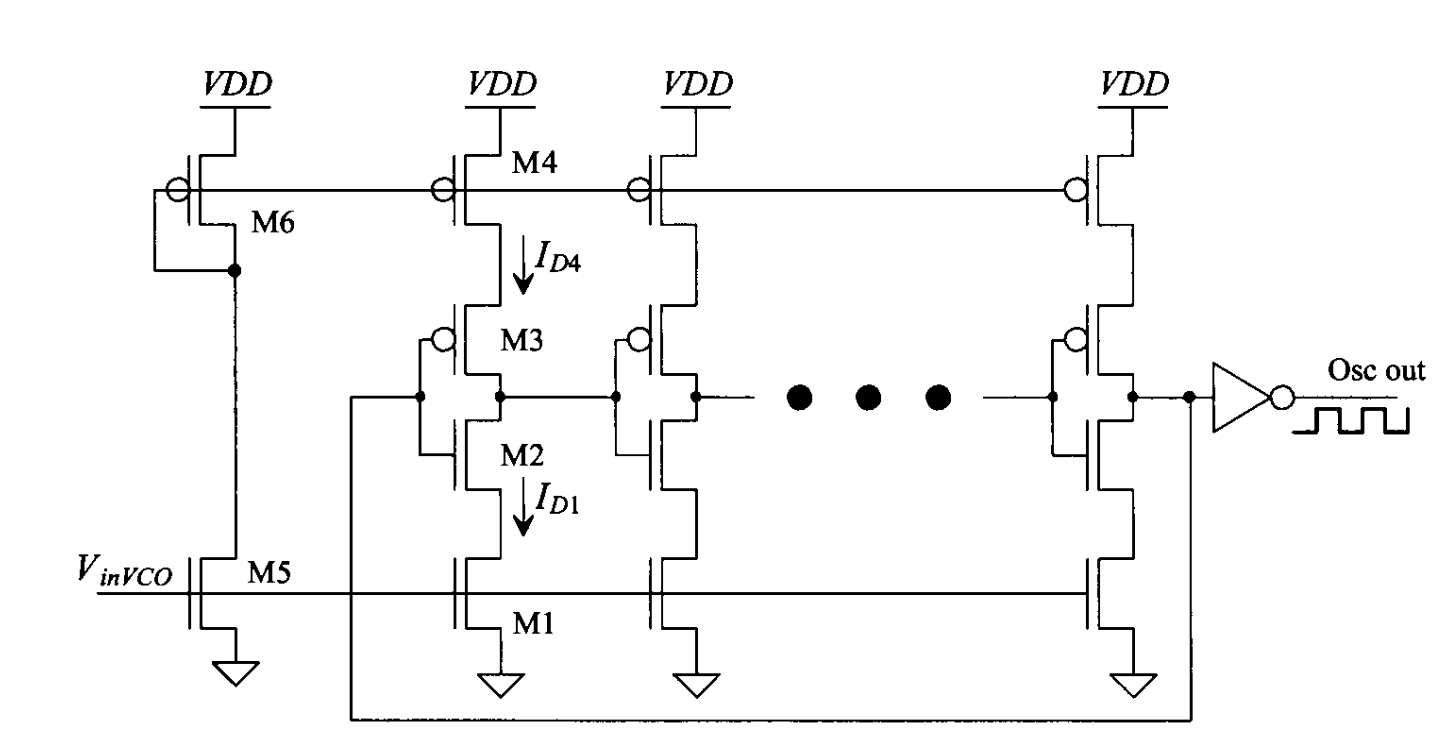
\includegraphics[0.6\textwidth]{figs/cs_vco_design.png}
\begin{figure}[h]
	\centering
	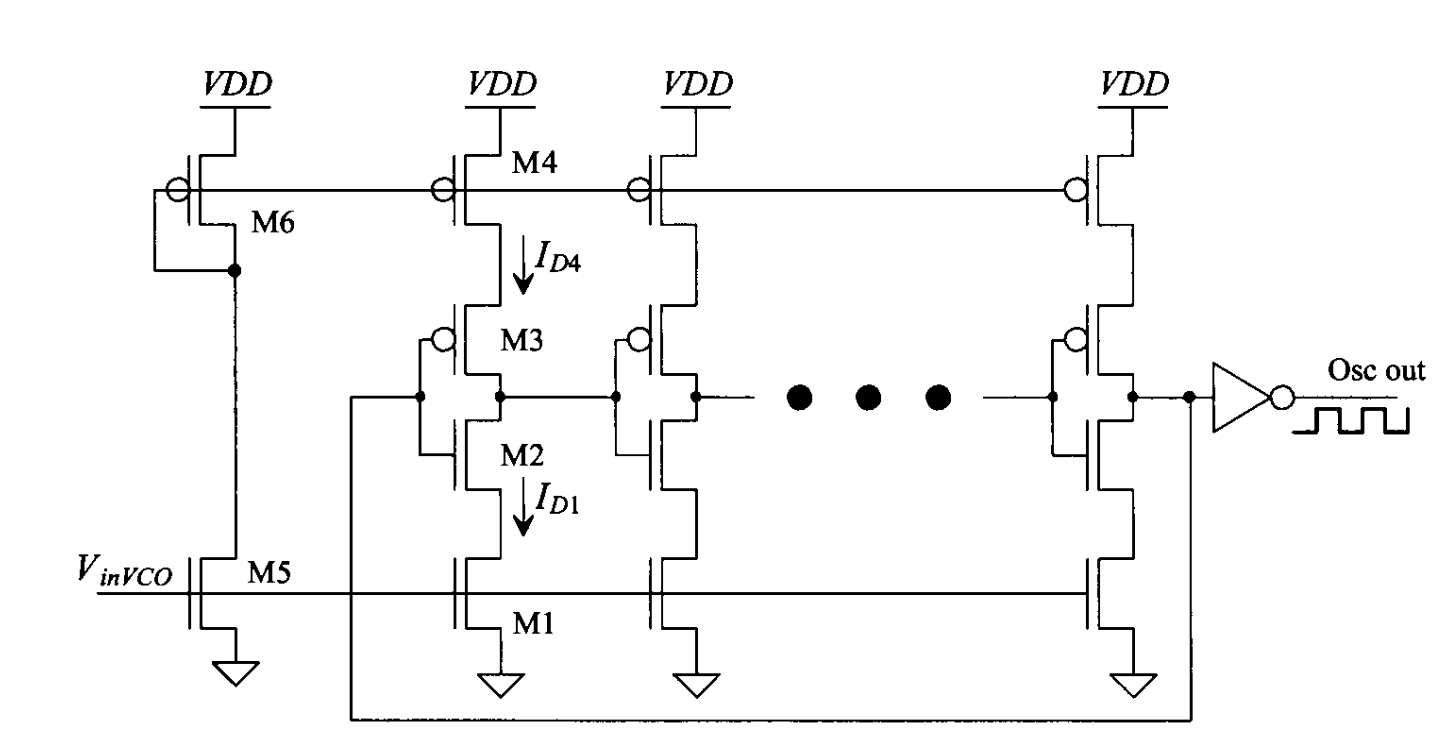
\includegraphics[width=0.5\textwidth]{figs/cs_vco_design.png}
	% \vspace{-0.3cm}
	\caption{Current Starved VCO Design}
	\label{fig:cs_vco_design}
	\vspace{0.5cm}
\end{figure}
\begin{figure}[h]
	\centering
	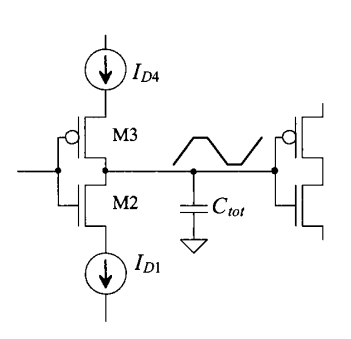
\includegraphics[width=0.5\textwidth]{figs/vco_simplified.png}
	% \vspace{-0.3cm}
	\caption{Simplified view of a single stage of the current-starved VCO}
	\label{fig:vco_simplified}
\end{figure}

To determine the design equations for use with the current-starved VCO, consider
the simplified schematic of one stage of the VCO fig \ref{fig:vco_simplified}. The total
capacitance on the drains of M2 and M3 is given by
\begin{equation}
	C_{\text{total}} = C_{\text{out}} + C_{\text{in}} = 
\underbrace{C'_{\text{ox}}(W_p L_p + W_n L_n)}_{\text{C\textsubscript{out}}} + 
\underbrace{\frac{3}{2} C'_{\text{ox}}(W_p L_p + W_n L_n)}_{\text{C\textsubscript{in}}}
\end{equation}
which is simply the output and input capacitances of the inverter. This equation can be written in a more useful form as
\begin{equation}
C_{\text{tot}} = \frac{5}{2} C'_{\text{ox}} (W_p L_p + W_n L_n)
\tag{19.19}
\end{equation}

\noindent The time it takes to charge $C_{\text{total}}$ from zero to $V_{SP}$ with the constant-current $I_{D4}$ is given by
\begin{equation}
t_1 = C_{\text{tot}} \cdot \frac{V_{SP}}{I_{D4}}
\tag{19.20}
\end{equation}

\noindent while the time it takes to discharge $C_{\text{total}}$ from $V_{DD}$ to $V_{SP}$ is given by
\begin{equation}
t_2 = C_{\text{tot}} \cdot \frac{V_{DD} - V_{SP}}{I_{D1}}
\tag{19.21}
\end{equation}

If we set $I_{D4} = I_{D1} = I_D$ (which we will label $I_{\text{Dcenter}}$ when $V_{\text{inVCO}} = V_{DD}/2$), then the sum of $t_1$ and $t_2$ is simply
\begin{equation}
t_1 + t_2 = \frac{C_{\text{tot}} \cdot V_{DD}}{I_D}
\tag{19.22}
\end{equation}

The oscillation frequency of the current-starved VCO for $N$ (an odd number $\geq 5$) of stages is
\begin{equation}
f_{\text{osc}} = \frac{1}{N(t_1 + t_2)} = \frac{I_D}{N \cdot C_{\text{tot}} \cdot V_{DD}}
\tag{19.23}
\end{equation}

which is $f_{\text{center}}(@ V_{\text{inVCO}} = V_{DD}/2 \text{ and } I_D = I_{\text{Dcenter}})$

firstly we have designed the Inverter stages and sized them accordingly and cascaded them to our required and connected a current Mirror to all the stages as in the Fig \ref{fig:vco_circuit}. The current mirror is used to control the current flowing through the inverter stages and thus control the frequency of oscillation. The output of the VCO is taken from the output of the last inverter stage. The VCO is designed to operate at a frequency of 1 GHz.
\begin{figure}[h]
	\centering
	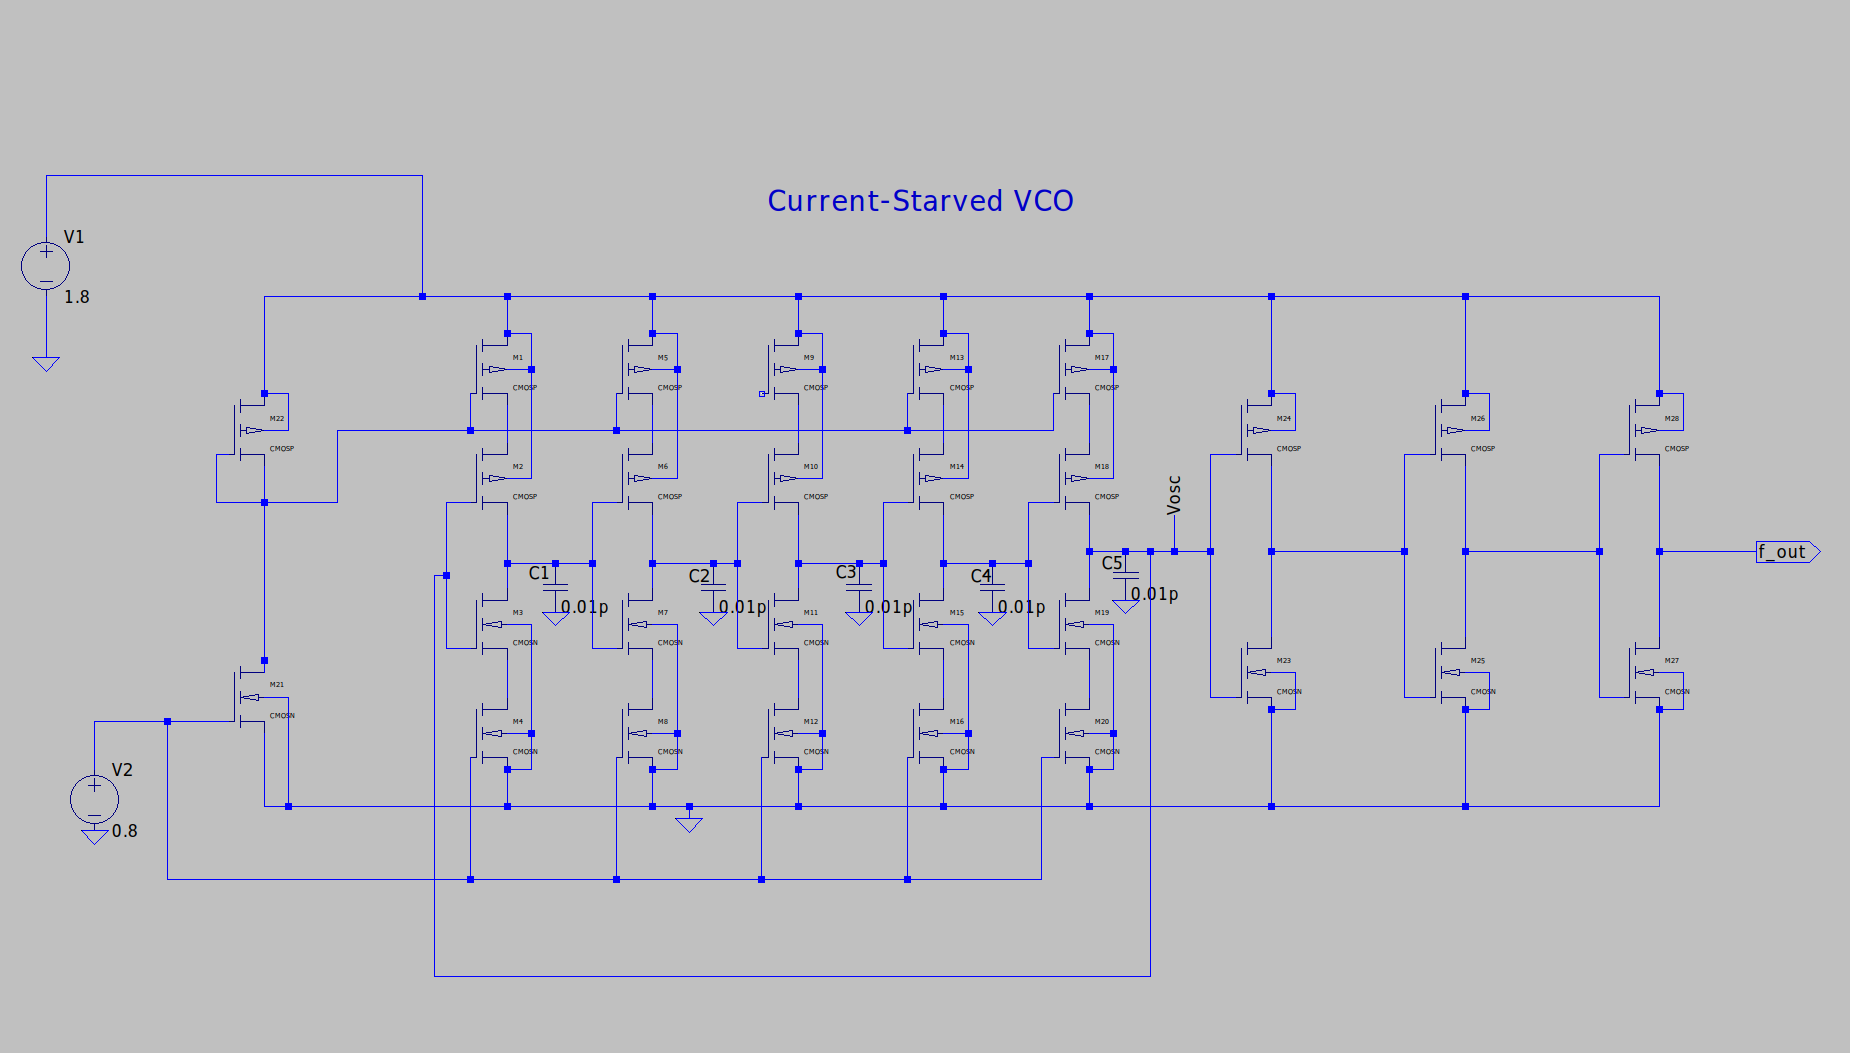
\includegraphics[width=0.9\textwidth]{figs/vco_c.png}
	% \vspace{-0.3cm}
	\caption{Current Starved VCO Circuit}
	\label{fig:vco_circuit}
	\vspace{0.5cm}
\end{figure}\\
The VCO ouput is not inherently a square wave (refer fig:\ref{fig:vco_op_c}) due to non-Ideal charachteristic of inverter here the ouput of the VCO is a irregular triangular wave. The output of the VCO is fed to a buffer and an inverter to convert the  of triangular wave to a square wave.
\begin{figure}
	\centering
	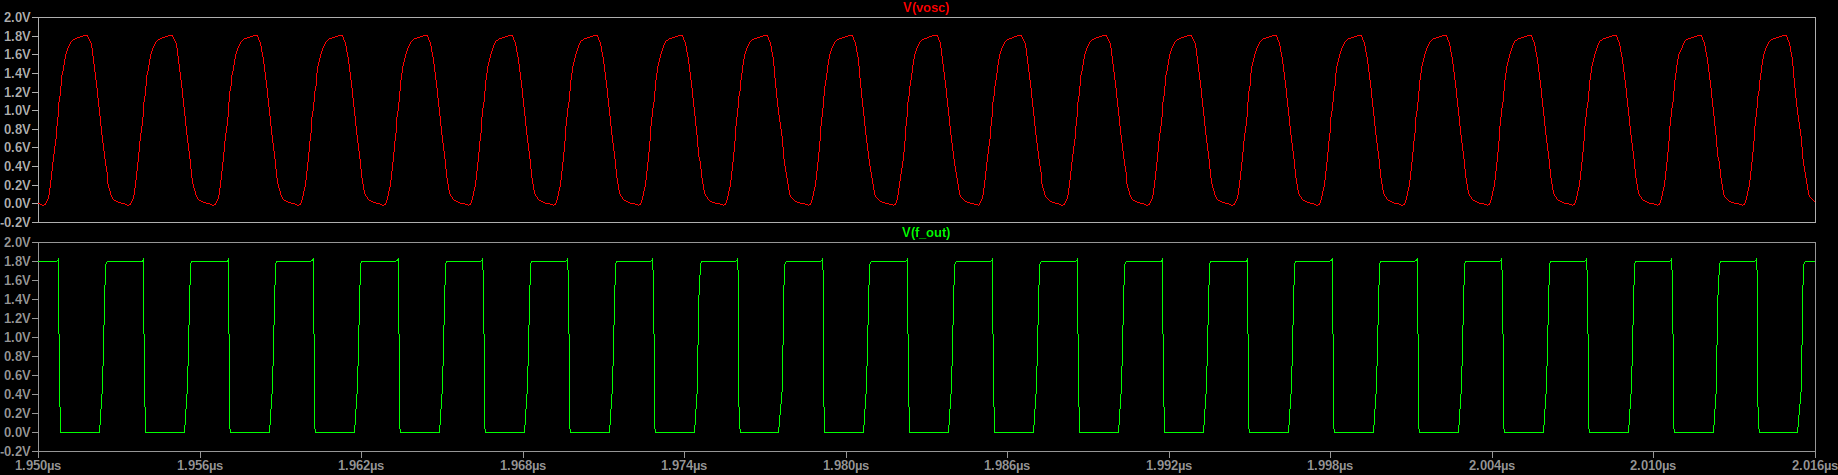
\includegraphics[width=0.9\textwidth]{figs/vco_op_both.png}
	% \vspace{-0.3cm}
	\caption{VCO output waveform before and after buffer+inverter}
	\label{fig:vco_op_c}
	\vspace{0.5cm}
\end{figure}
In Figure \ref{fig:vco_sim}, the Transient analysis of circuit in Figure \ref{fig:vco_circuit} is shown.
\begin{figure}[H]
	\centering
	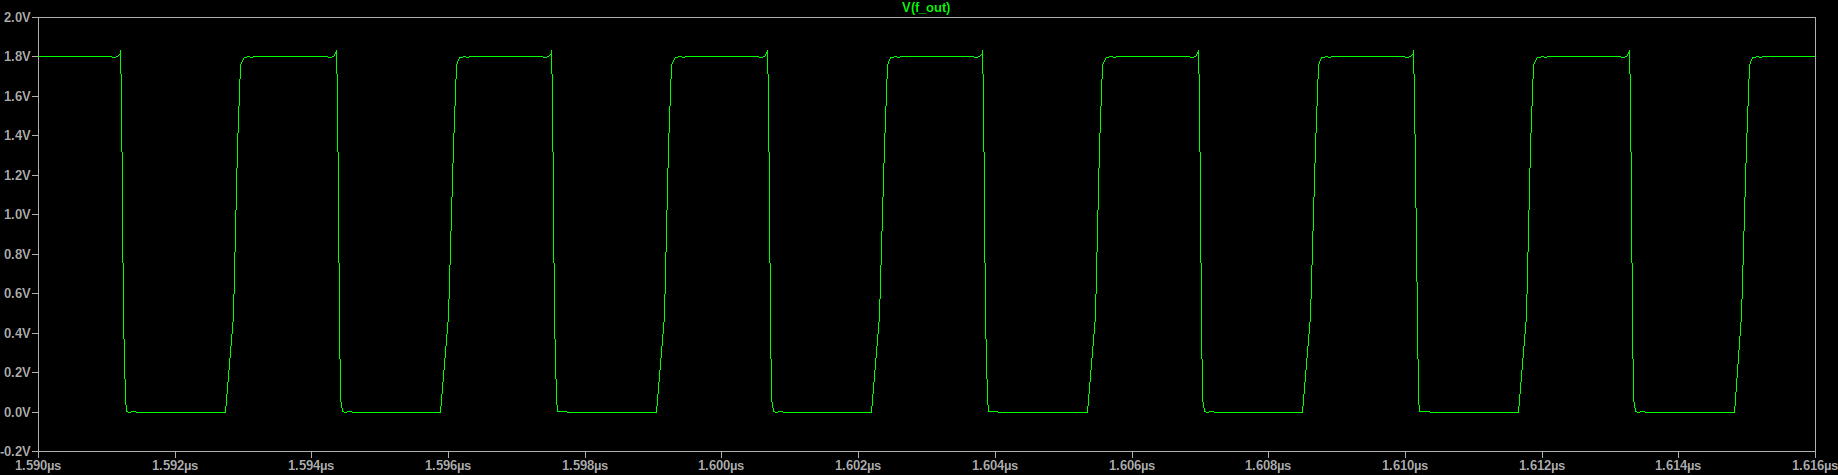
\includegraphics[width=0.9\textwidth]{figs/vco_op1.png}
	% \vspace{-0.3cm}
	\caption{output waveform of VCO}
	\label{fig:vco_sim}
\end{figure}

\subsection{Frequency Divider Design}
\label{sec:freq_div}
\subsection{Complete PLL Design}
\label{sec:complete_pll}

